% \documentclass{article}

% % Recommended, but optional, packages for figures and better typesetting:
% \usepackage{microtype}
% \usepackage{graphicx}
% % \usepackage{subfigure}
% \usepackage{booktabs} % for professional tables
% \usepackage{subcaption}
% \usepackage[noend]{algpseudocode}
% \usepackage{enumitem}
% \usepackage{amsmath}
% \usepackage{amssymb}

% % hyperref makes hyperlinks in the resulting PDF.
% % If your build breaks (sometimes temporarily if a hyperlink spans a page)
% % please comment out the following usepackage line and replace
% % \usepackage{icml2021} with \usepackage[nohyperref]{icml2021} above.
% \usepackage{hyperref}

% % Attempt to make hyperref and algorithmic work together better:
% \newcommand{\theHalgorithm}{\arabic{algorithm}}
% \usepackage{multirow}

% % Use the following line for the initial blind version submitted for review:
% \usepackage{icml2021}
% % operators

% \newcommand{\argmax}{\operatornamewithlimits{argmax}}
% \newcommand{\argmin}{\operatornamewithlimits{argmin}}

% vectors
\let\avec\vec
%\renewcommand{\vec}[1]{\ensuremath{\boldsymbol{#1}}}
\renewcommand{\v}[1]{\ensuremath{\boldsymbol{#1}}}

\newcommand{\src}{\lstinline[mathescape, keepspaces]}
\newcommand{\msrc}[1]{\mbox{\src!#1!}}

% \newcommand{\tens}[1]{%
%   \mathbin{\mathop{\otimes}\limits_{#1}}%
% }

% symbol shorthands (lowercase)
\newcommand{\x}{\ensuremath{\v{x}}}
\newcommand{\y}{\ensuremath{\v{y}}}
\newcommand{\z}{\ensuremath{\v{z}}}
\newcommand{\h}{\v{\eta}}
\newcommand{\e}{\v{\epsilon}}
\renewcommand{\u}{\v{u}}
\newcommand{\pd}{\ensuremath{\partial}}
% \newcommand{\x}{\ensuremath{x}}
% \newcommand{\y}{\ensuremath{y}}
% \newcommand{\z}{\ensuremath{z}}
% \newcommand{\h}{\ensuremath{\eta}}
% \newcommand{\e}{\ensuremath{\epsilon}}
\renewcommand{\u}{\ensuremath{u}}
\newcommand{\q}{\theta}
\newcommand{\f}{\phi}
\renewcommand{\l}{\lambda}
\renewcommand{\t}{\tau}

% symbol shorthands (uppercase)
\renewcommand{\L}{\ensuremath{\mathcal{L}}}
% \newcommand{\KL}[2]{\ensuremath{\mathrm{KL}\left({#1} \:\middle\vert\middle\vert\: {#2}\right)}}
\newcommand{\E}{\ensuremath{\mathbb{E}}}
\newcommand{\N}{\ensuremath{\mathcal{N}}}
\newcommand{\C}{\ensuremath{\mathtt{Concrete}}}

%\let\lmid\mid
%\renewcommand{\mid}{\!\lmid\!}

\newcommand{\eval}{\ensuremath{$\reflectbox{$\,\leadsto\,$}$}}
%\newcommand{\eval}{\sim}
\newcommand{\hide}[1]{}

\makeatletter
\DeclareRobustCommand{\cev}[1]{%
  \mathpalette\do@cev{#1}%
}
\newcommand{\do@cev}[2]{%
  \fix@cev{#1}{+}%
  \reflectbox{$\m@th#1\vec{\reflectbox{$\fix@cev{#1}{-}\m@th#1#2\fix@cev{#1}{+}$}}$}%
  \fix@cev{#1}{-}%
}
\newcommand{\fix@cev}[2]{%
  \ifx#1\displaystyle
    \mkern#23mu
  \else
    \ifx#1\textstyle
      \mkern#23mu
    \else
      \ifx#1\scriptstyle
        \mkern#22mu
      \else
        \mkern#22mu
      \fi
    \fi
  \fi
}

% % If accepted, instead use the following line for the camera-ready submission:
% %\usepackage[accepted]{icml2021}

% % The \icmltitle you define below is probably too long as a header.
% % Therefore, a short form for the running title is supplied here:
% \icmltitlerunning{Supplementary Materials}

% \begin{document}
\newpage
\onecolumn
\icmltitle{Supplementary Materials}
\appendix
\section{Model Architectures}
\label{appendix-architectures}
Table~\ref{appendex:tab:arch-cebm}, Table~\ref{appendex:tab:arch-vae}, and Table~\ref{appendex:tab:arch-igebm} show the architectures used for CEBM, VAE, and IGEBM, respectively.

\begin{table}[!h]
\caption{Architecture of CEBM}
    \centering
    \begin{subtable}[h]{.5\linewidth}
    \caption{MNIST and Fashion-MNIST.}
    \centering
        \begin{tabular}{|l|}
        \toprule
        \textbf{Encoder} \\
        \midrule
        Input $28\times28\times1$ images  \\
        \hline 
        $3\times3$ conv. 64 LeakyReLU. stride 1. padding 1  \\
        \hline 
        $4\times4$ conv. 64 LeakyReLU. stride 2. padding 1 \\
        \hline 
        $4\times4$ conv. 32 LeakyReLU. stride 2. padding 1  \\
        \hline
        $4\times4$ conv. 32 LeakyReLU. stride 2. padding 1 \\
        \hline
        FC. 128 LeakyReLU \\
        \hline
        FC. $2\times128$ \\
        \bottomrule
        \end{tabular}
    \end{subtable}%%%
    \begin{subtable}[h]{.5\textwidth}
    \caption{CIFAR10 and SVHN.}
    \centering
        \begin{tabular}{|l|}
        \toprule
        \textbf{Encoder}  \\
        \midrule
        Input $32\times32\times3$ images  \\
        \hline 
        $3\times3$ conv. 64 LeakyReLU. stride 1. padding 1  \\
        \hline 
        $4\times4$ conv. 128 LeakyReLU. stride 2. padding 1 \\
        \hline 
        $4\times4$ conv. 256 LeakyReLU. stride 2. padding 1  \\
        \hline
        $4\times4$ conv. 512 LeakyReLU. stride 2. padding 1  \\
        \hline
        FC. 128 LeakyReLU \\
        \hline
        FC. $2\times128$\\
        \bottomrule
        \end{tabular}
    \vspace*{1ex}
    \end{subtable}
    \label{appendex:tab:arch-cebm}
\end{table}



% \newpage
\begin{table}[!h]
\caption{Architecture of VAE}
    \centering
    \begin{subtable}[h]{\textwidth}
    \caption{MNIST and Fashion-MNIST.}
    \centering
        \begin{tabular}{|l|l|}
        \toprule
        \textbf{Encoder} & \textbf{Decoder} \\
        \midrule
        Input $28\times28\times1$ images & Input $z\in \mathbb{R}^{128}$ latent variables \\
        \hline 
        $3\times3$ conv. 64 LeakyReLU. stride 1. padding 1 & FC. 128 ReLU \\
        \hline 
        $4\times4$ conv. 64 LeakyReLU. stride 2. padding 1 & FC. $3\times3\times32$ ReLU \\
        \hline 
        $4\times4$ conv. 32 LeakyReLU. stride 2. padding 1 & $4\times4$ upconv. 32 LeakyReLU. stride 2. padding 1 \\
        \hline
        $4\times4$ conv. 32 LeakyReLU. stride 2. padding 1 & $4\times4$ upconv. 64 LeakyReLU. stride 2. padding 1 \\
        \hline
        FC. 128 ReLU & $4\times4$ upconv. 64 LeakyReLU. stride 2. padding 0 \\
        \hline
        FC. $2\times128$ & $3\times3$ upconv. 1 stride 1. padding 0 \\
        \bottomrule
        \end{tabular}
    \vspace*{1ex}
    \end{subtable}
    \begin{subtable}[h]{\textwidth}
    \caption{CIFAR10 and SVHN.}
    \centering
        \begin{tabular}{|l|l|}
        \toprule
        \textbf{Encoder} & \textbf{Decoder} \\
        \midrule
        Input $32\times32\times3$ images & Input $z\in \mathbb{R}^{128}$ latent variables \\
        \hline 
        $3\times3$ conv. 64 LeakyReLU. stride 1. padding 1 & FC. 128 ReLU \\
        \hline 
        $4\times4$ conv. 128 LeakyReLU. stride 2. padding 1 & FC. $4\times4\times512$ ReLU \\
        \hline 
        $4\times4$ conv. 256 LeakyReLU. stride 2. padding 1 & $4\times4$ upconv. 32 LeakyReLU. stride 2. padding 1 \\
        \hline
        $4\times4$ conv. 512 LeakyReLU. stride 2. padding 1 & $4\times4$ upconv. 64 LeakyReLU. stride 2. padding 1 \\
        \hline
        FC. 128 ReLU & $3\times3$ upconv. 64 LeakyReLU. stride 2. padding 1 \\
        \hline
        FC. $2\times128$ & $3\times3$ upconv. 1 stride 1. padding 1 \\
        \bottomrule
        \end{tabular}
    \vspace*{1ex}
    \end{subtable}
    \label{appendex:tab:arch-vae}
\end{table}

\begin{table}[!h]
\caption{Architecture of IGEBM}
    \centering
    \begin{subtable}[h]{.5\textwidth}
    \caption{MNIST and Fashion-MNIST.}
    \centering
        \begin{tabular}{|l|}
        \toprule
        \textbf{Encoder} \\
        \midrule
        Input $28\times28\times1$ images  \\
        \hline 
        $3\times3$ conv. 64 LeakyReLU. stride 1. padding 1  \\
        \hline 
        $4\times4$ conv. 64 LeakyReLU. stride 2. padding 1 \\
        \hline 
        $4\times4$ conv. 32 LeakyReLU. stride 2. padding 1  \\
        \hline
        $4\times4$ conv. 32 LeakyReLU. stride 2. padding 1 \\
        \hline
        FC. 128 LeakyReLU \\
        \hline
        FC. 128 LeakyReLU. FC. 1 \\
        \bottomrule
        \end{tabular}
    \end{subtable}%%%
    \begin{subtable}[h]{.5\textwidth}
    \caption{CIFAR10 and SVHN.}
    \centering
        \begin{tabular}{|l|}
        \toprule
        \textbf{Encoder}  \\
        \midrule
        Input $32\times32\times3$ images  \\
        \hline 
        $3\times3$ conv. 64 LeakyReLU. stride 1. padding 1  \\
        \hline 
        $4\times4$ conv. 128 LeakyReLU. stride 2. padding 1 \\
        \hline 
        $4\times4$ conv. 256 LeakyReLU. stride 2. padding 1  \\
        \hline
        $4\times4$ conv. 512 LeakyReLU. stride 2. padding 1  \\
        \hline
        FC. 128 LeakyReLU \\
        \hline
        FC. 128 LeakyReLU. FC. 1\\
        \bottomrule
        \end{tabular}
    \vspace*{1ex}
    \end{subtable}
    \label{appendex:tab:arch-igebm}
\end{table}

\section{Training Details}
\label{appendix-sec:training-details}
In CEBMs and VAEs, we choose the dimension of latent variables to be 128. For CEBMS, We found that the optimization becomes difficult with smaller dimensions. We L2 regularize energy magnitudes (proposed by~\citet{du2019implicit}), where the coefficient of the L2 regularization term is 0.1. We empirically found that the training would become unstable without this regularization. We train our models using 60 SGLD steps where we initialize samples from the replay buffer with 0.95 probability, and initialize from uniform noise with 0.05 probability. We train all the models with 90k gradient steps, batch size 128, Adam optimizer with learning rate 1e-4. When doing PCD, we used a reply buffer of size 5000. We set the $\alpha$ in the SGLD teps to be 0.075. Similar to~\citet{du2019implicit}, we found it useful to add some noise to the image before encoding. In our experiments, we used Gaussian noise with $\sigma^{2} = 0.03$. For the mixture models (CEBMM and GMM-VAE), we used 50 mixtures.  

\newpage
\section{Additional Results}
\label{app:sec:additional-results}

\subsection{Confusion Matrices on 1-NN Classification}
\label{appendix-sec:confuion matrices}
We perform 1-nearest-neighbor classification task for MNIST, Fashion-MNIST, SVHN, CIFAR10. We compute the L2 distance in the latent space of VAE, IGEBM and CEBM, and also in pixel space. We visualize the confusion matrices
\begin{figure}[!h]
\centering
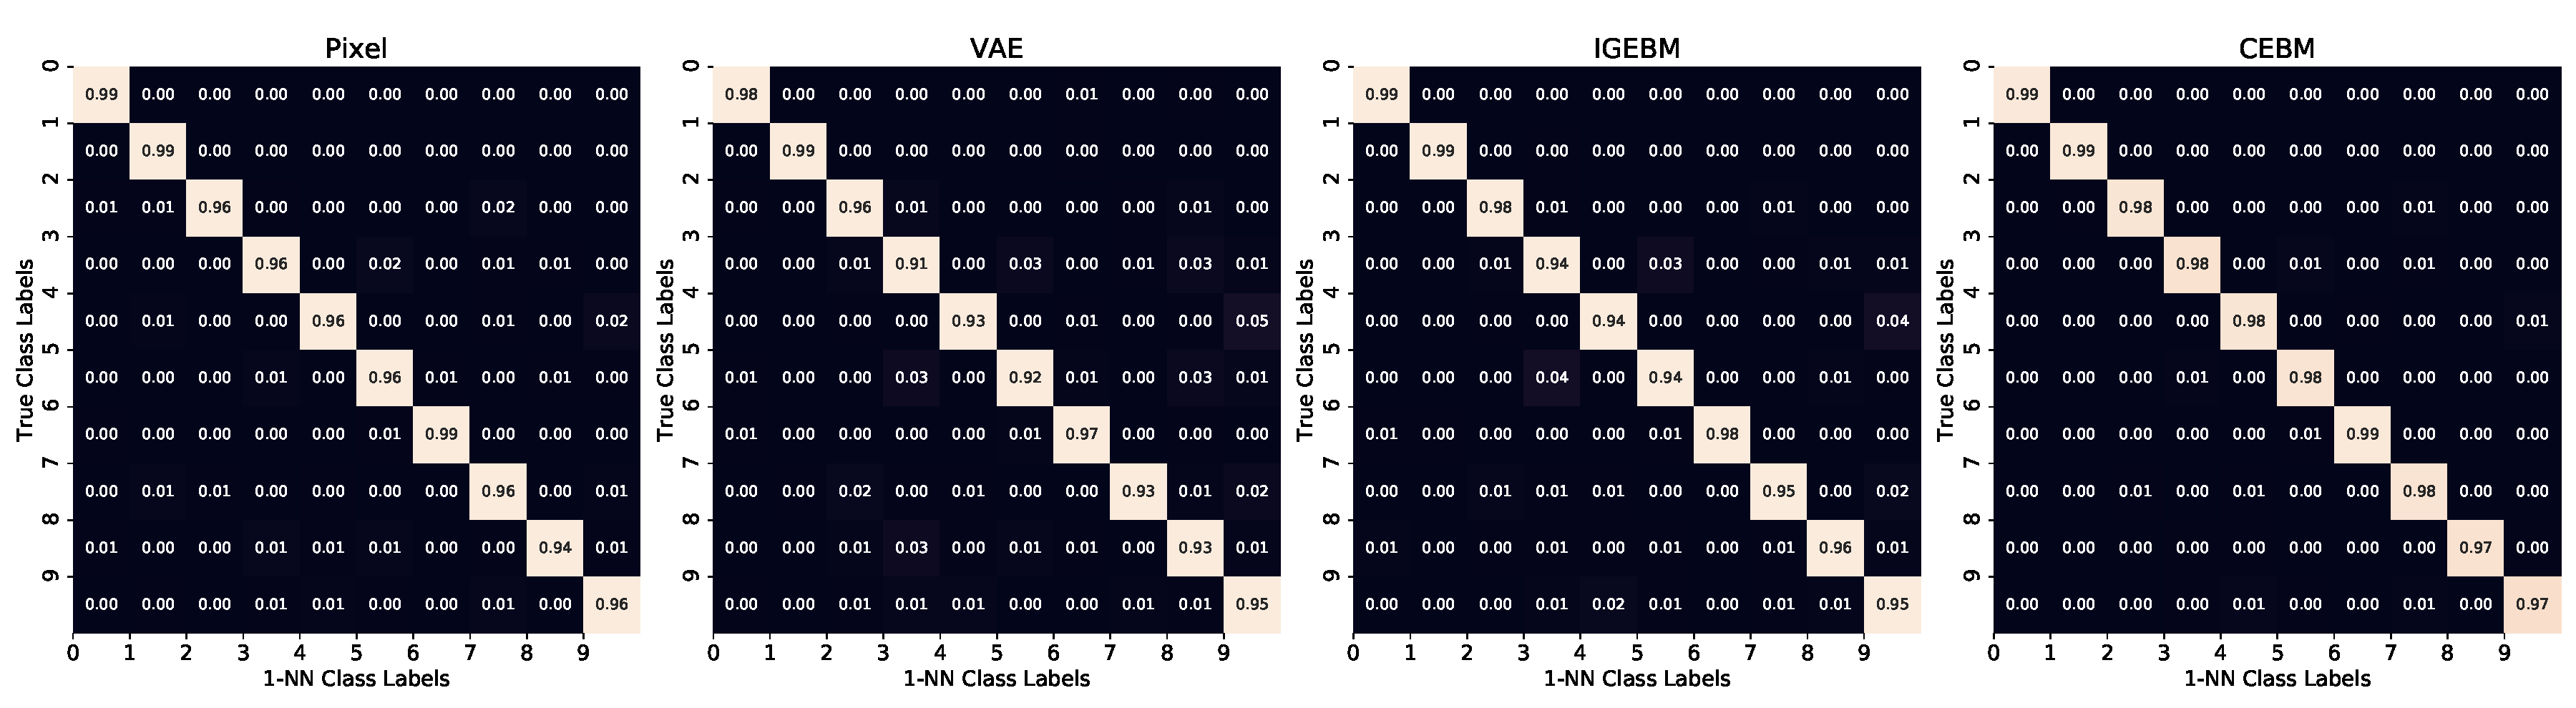
\includegraphics[width=\linewidth]{figures/confusion_matrix_14row_mnist.pdf}
\caption{MNIST}
\label{appendix:confusion-matrices-mnist}
\end{figure}
\begin{figure}[!h]
\centering
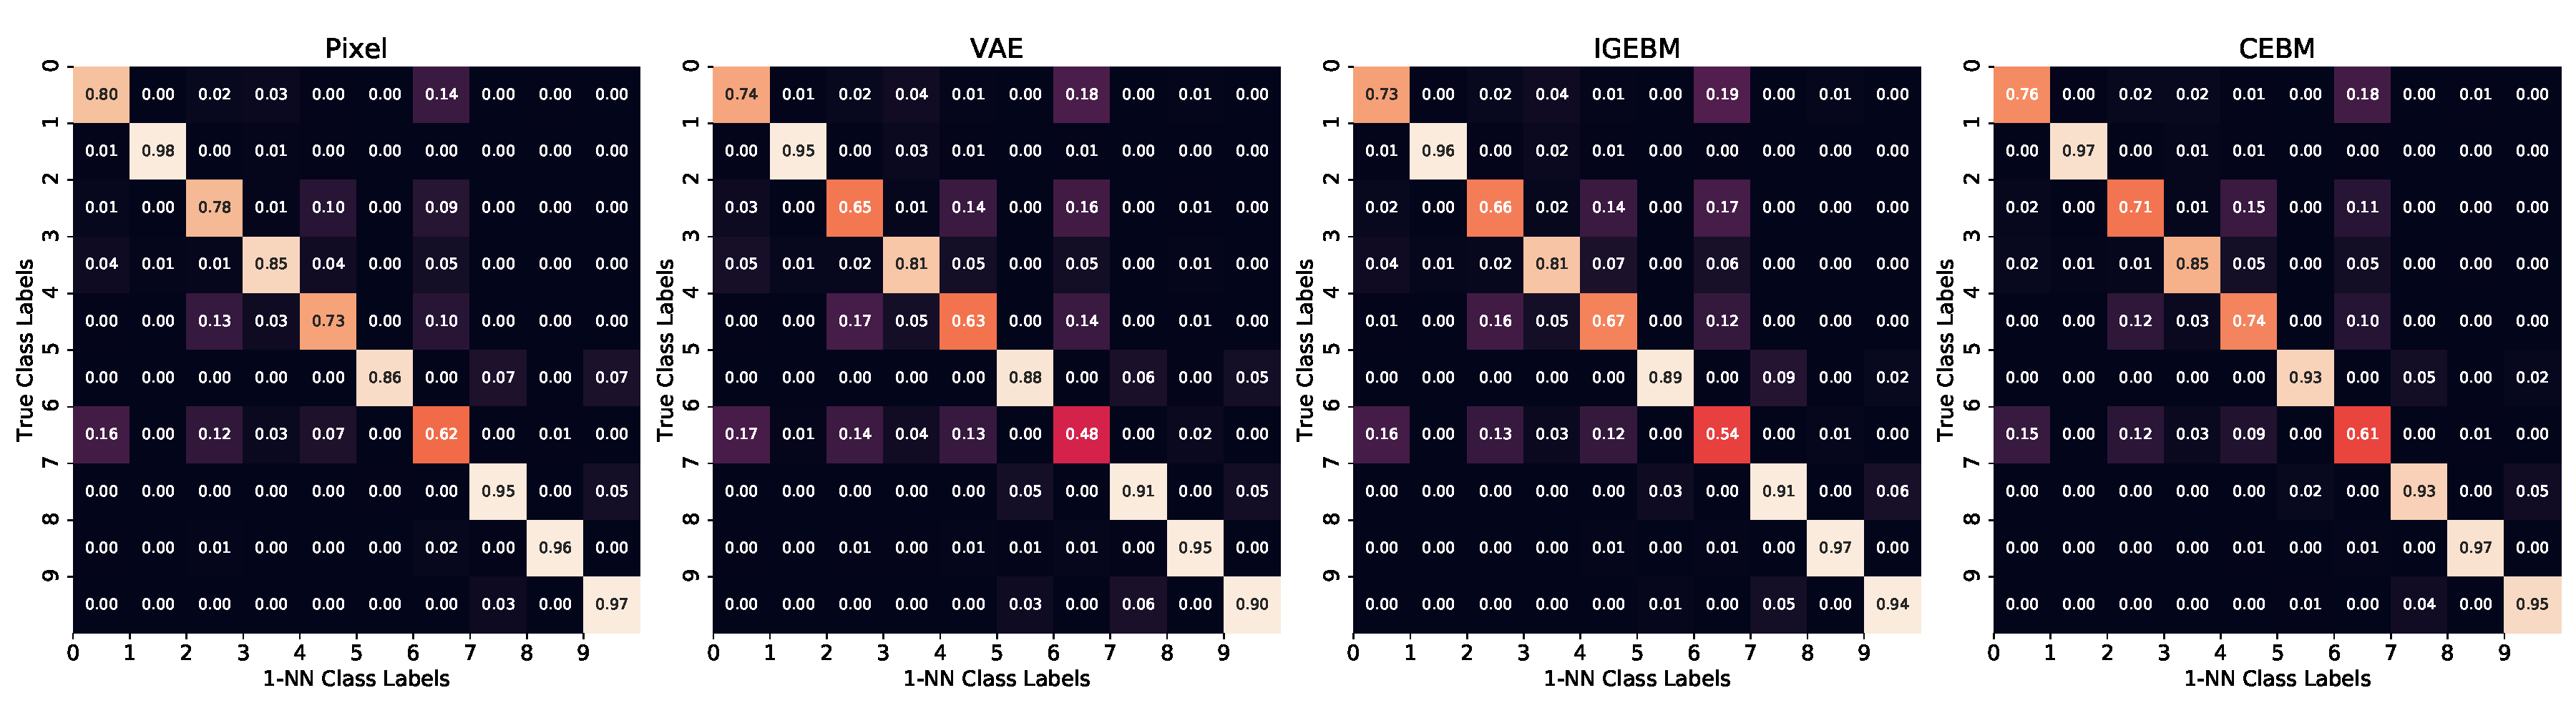
\includegraphics[width=\linewidth]{figures/confusion_matrix_14row_fashionmnist.pdf}
\caption{Fashion-MNIST}
\label{appendix:confusion-matrices-fmnist}
\end{figure}
\vspace{-2em}
\begin{figure}[!h]
\centering
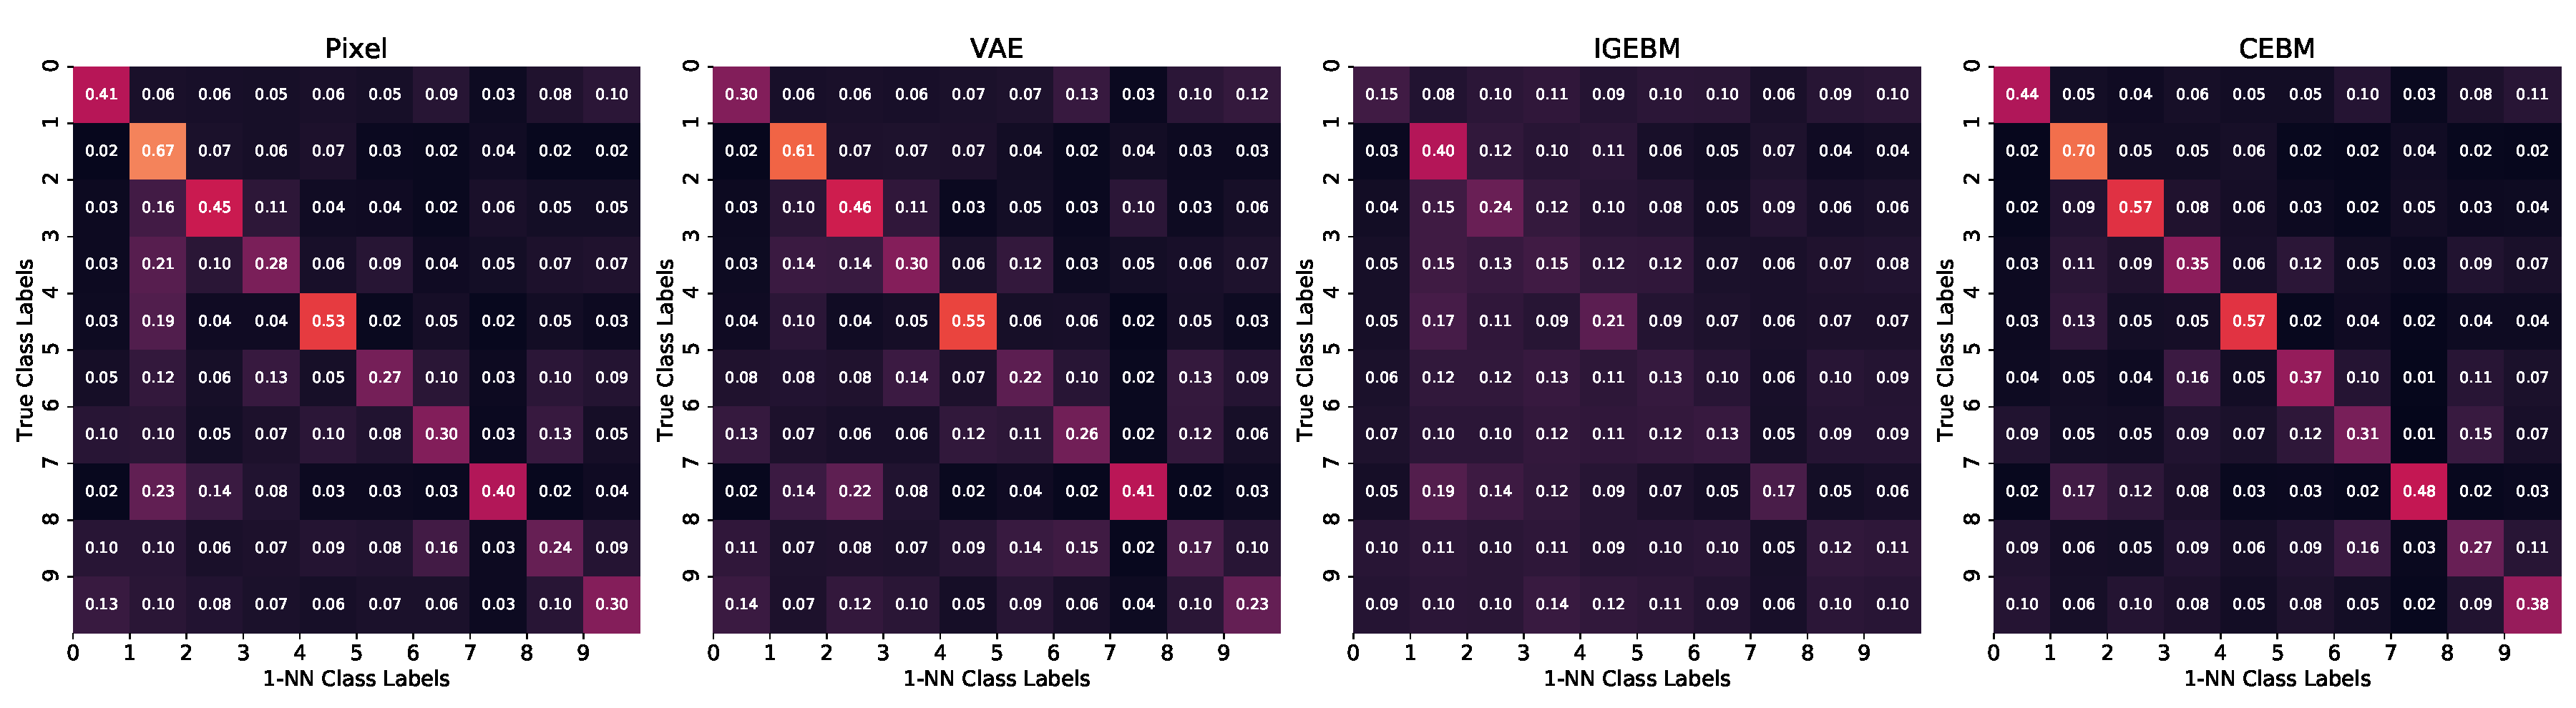
\includegraphics[width=\linewidth]{figures/confusion_matrix_14row_svhn.pdf}
\caption{SVHN}
\label{appendix:confusion-matrices-svhn}
\end{figure}
\vspace{-2em}
\begin{figure}[!h]
\centering
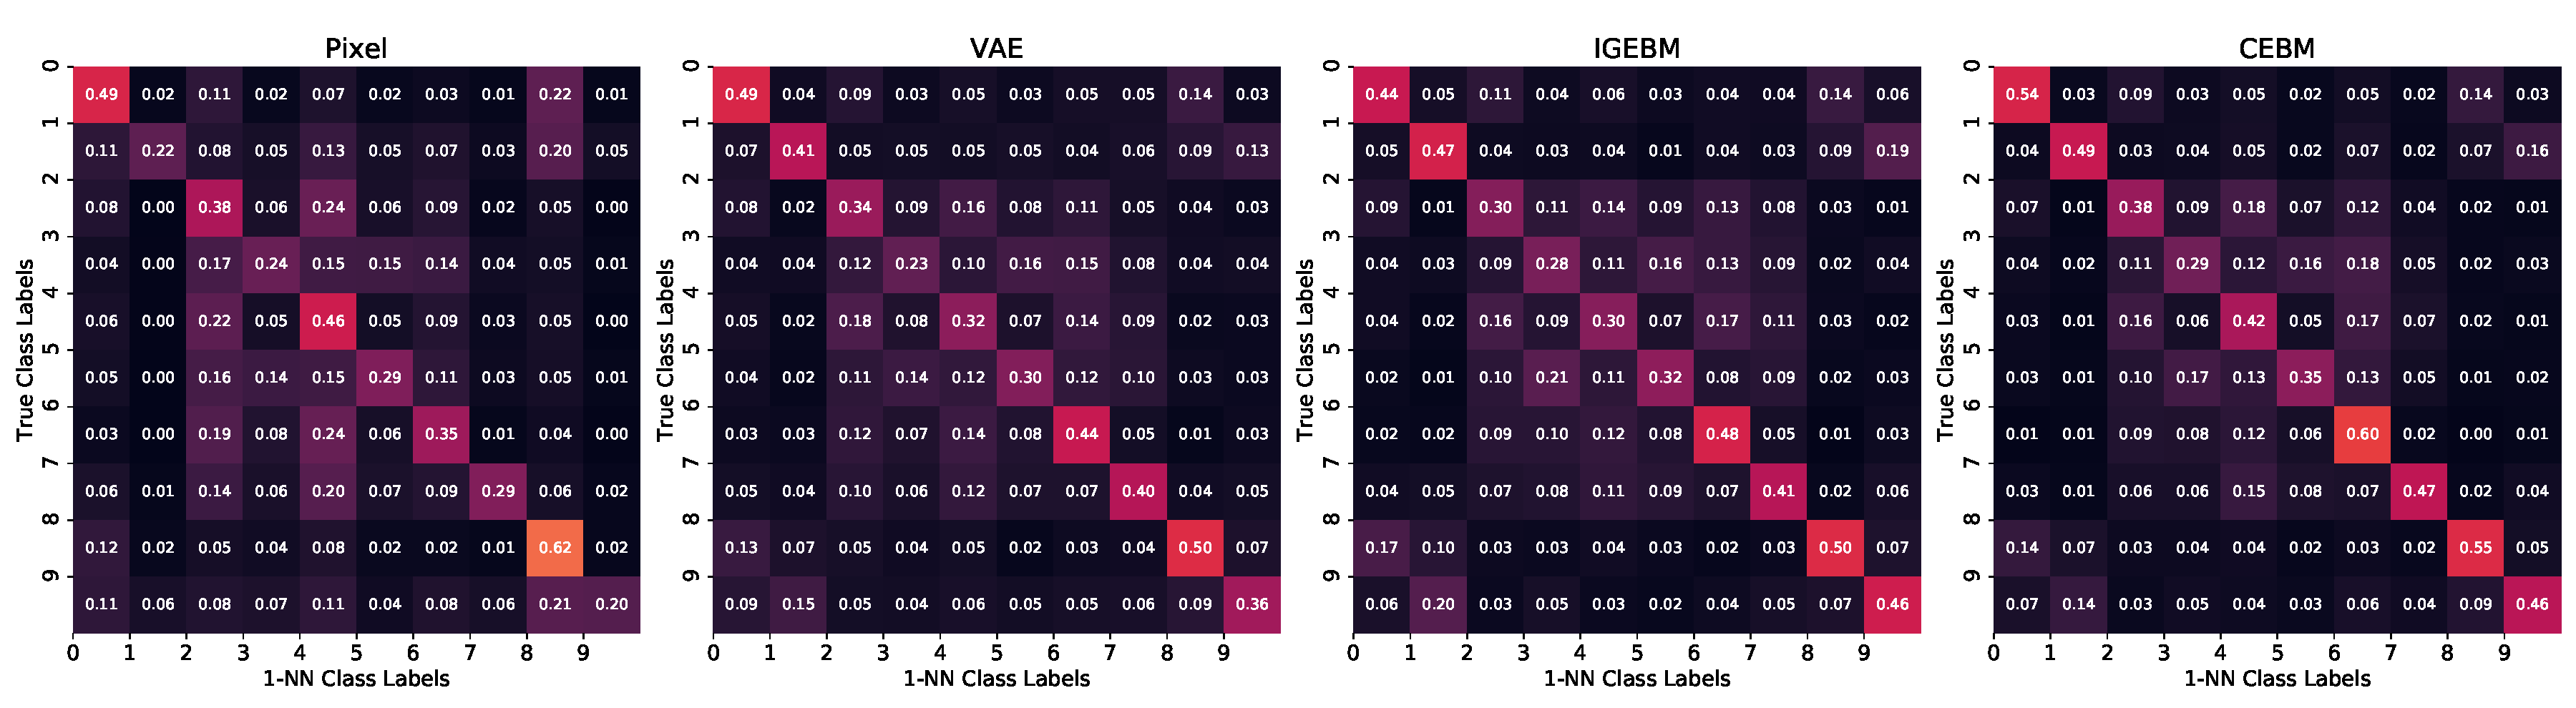
\includegraphics[width=\linewidth]{figures/confusion_matrix_14row_cifar10.pdf}
\caption{CIFAR10}
\label{appendix:confusion-matrices-cifar10}
\end{figure}

\newpage
\subsection{Out-of-Distribution Detection}
\label{appendix-sec:ood-detection}
We compute the AUROC score in OOD detection based on two different score functions.
\setlength{\tabcolsep}{4.5pt}
\begin{table*}[!h]
\caption{AUROC scores in OOD Detection. We use $\log p_{\q}(\x)$ and $\| \nabla_{\x}\log p_{\q}(\x)\|$ as score functions.The left block shows results of the models trained on F-MNIST and tested on MNIST, E-MNIST, Constant (C); The right block shows results of the models trained on CIFAR-10 and tested on SVHN, Texture and Constant (C).}
\centering
\begin{tabular}{l|ccc|ccc||ccc|ccc}
\toprule
& \multicolumn{6}{c||}{Fashion-MNIST} &    \multicolumn{6}{c}{CIFAR-10}\\
& \multicolumn{3}{c|}{$\log p_{\q}(\x)$} & \multicolumn{3}{c||}{$\| \nabla_{\x}\log p_{\q}(\x)\|$} &  \multicolumn{3}{c|}{$\log p_{\q}(\x)$} & \multicolumn{3}{c}{$\| \nabla_{\x}\log p_{\q}(\x)\|$}\\
\midrule
            &  MNIST  & E-MNIST& C &  MNIST & E-MNIST & C &  SVHN & Texture & C &  SVHN & Texture & C \\
\midrule
VAE         & .50 & .39 & .9 & .61 & .57 & .1  & .42 & \textbf{.58} & .41 & .38 & \textbf{.51} & .37 \\
IGEBM       & .35 & .36 & .90 & .78 & .82 & .96& .45 & .31 & .64 & .33 & .17 & \textbf{.62} \\
CEBM        & .37 & .34 & .90 & \textbf{.82} & \textbf{.89} & \textbf{.98} & .47 & .32 & \textbf{.66} & .31 & .17 & .54 \\
CEBMM       & \textbf{.56} & \textbf{.56} & \textbf{.92} & .56 & .80 & .95     & \textbf{.55} & .30 & .62 & \textbf{.40} & .23 & \textbf{.62}  \\
\bottomrule
\end{tabular}
\label{app:tab:ood-detection}
\end{table*}
% \end{document}

\begin{algorithm}[!t]
\caption{Persistent Contrastive Divergence}
\label{alg:cebm}
\begin{algorithmic}[1]
\State \textbf{input:} $p_\text{data}(\cdot)$, $\q$, $\alpha$, $T$
\State $\mathcal{B} \gets \{x_b \sim \mathcal{U} \text{ \textbf{for}}\ b = 1 \ldots \text{buffer-size} \}$
\While{not converged}
\State $x \sim p_\text{data}(x)$
\State $x' \sim \mathcal{B}$ with 95\% probability and $\mathcal{U}$ otherwise
\For{$t = 1 \ldots T$}
\State $\epsilon \sim \mathcal{N}(0, \alpha)$
\State $x' \gets x' - \frac{\alpha}{2} \nabla_{x} E_\q (x') + \epsilon$
\EndFor
% \State $\vx^{-} \gets \vx^{-}.\text{detach()} $
\State $\Delta_{\q} \gets \nabla_{\q} E_{\q}(x) - \nabla_{\q} E_\q(x')$  
\State $\q \gets \text{Adam}(\q, \Delta_{\q})$
\State $\mathcal{B}[x'] \gets x'$
\EndWhile
\State \textbf{return} $\q$
\end{algorithmic}
\end{algorithm}